\section{Příklad 3}
% Jako parametr zadejte skupinu (A-H)
\tretiZadani{B}

\subsection{Řešení}

Úkolem je stanovit napětí a proud rezistorem $R_4$ pomocí metody uzlových napětí. Uzly v obvodu si označíme písmeny $E, F, G, H$, a proudy v jednotlivých větvích si označíme podle příslušných rezistorů (viz obrázek).

\begin{figure}[H]
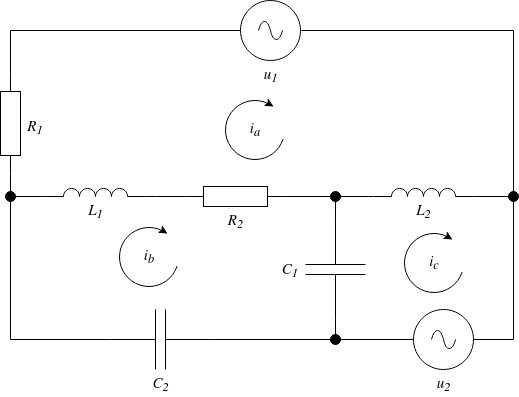
\includegraphics[scale=0.5]{Pr3/step1.png}
\centering
\caption{Označení proudů ve větvích obvodu}
\end{figure}

Nyní si rozepíšeme proudy $I_{R1}$ až $I_{R5}$ pomocí uzlových napětí:

$$ I_{R1} = \frac{U_a - U}{R_1} $$
$$ I_{R2} = \frac{U_b - U_a}{R_2} $$
$$ I_{R3} = \frac{U_a}{R_3} $$
$$ I_{R4} = \frac{U_b - U_c}{R_4} $$
$$ I_{R5} = \frac{U_c}{R_5} $$

Následně pro libovolné tři uzly sestavíme rovnice podle prvního Kirchoffova zákona, dle konvence, že vstupující proud má vždy záporné znaménko:

$$ F: \: I_{R2} + I_{R4} + I_2 = 0 $$
$$ G: \: I_{R5} + I_1 - I_{R4} - I_2 = 0 $$
$$ H: \: - I_{R1} - I_{R3} - I_{R5} - I_1 = 0 $$

Do těchto rovnic dosadíme výrazy získané v předchozím kroce, a roznásobíme zlomky:

$$ R_4U_B - R_4U_A + R_2U_B - R_2U_C + R_2R_4I_2 = 0 $$
$$ R_4U_C + R_4R_5I_1 - R_5U_B + R_5U_C - R_4R_5I_2 = 0 $$
$$ -R_3R_5U_A + R_3R_5U - R_1R_5U_A -R_1R_3U_C -R_1R_3R_5I_1 = 0 $$

Tyto rovnice převedeme do tvaru matice, dosadíme hodnoty ze zadání, a vyřešíme (celý postup zde neuvádím). Zajímají nás hodnoty $U_B$ a $U_C$, neboť napětí na rezistoru $R_4$ je rozdílem právě těchto napětí.

$$ \left (
\begin{array}{ccc|c}
	-R_4 & R_4 + R_2 & -R_2 & -R_2R_4I_2 \\
	0 & -R_5 & R_4 + R_5 & R_4R_5I_2 - R_4R_5I_1 \\
	-R_3R_5 - R_1R_5 & 0 & -R_1R_3 & R_1R_3R_5I_1 - R_3R_5U
\end{array}
\right) $$

Vyřešením této soustavy dostaneme hodnoty $U_B \doteq 14,0937 V$ a $U_C \doteq 8,7469 V$. Napětí $U_{R4}$ se rovná rozdílu těchto dvou napětí:

$$ U_{R4} = U_B - U_C \doteq 5,3469 V $$

Proud procházející rezistorem už zjistíme jednoduše pomocí Ohmova zákona:

$$ I_{R4} = \frac{U_{R4}}{R_4} \doteq 0,1573 A $$
